\documentclass{article}

%opening
\title{Simulating MRC, MRT, Alamouti\\in a Rayleigh Fading, MIMO Environment\\
\large Project \#4}
\author{Intelligent Communication Systems (ICS) Lab.\\노용재}
\date{Winter Intern Seminar (2023-1)}

\usepackage{kotex} % korean
\usepackage[margin=1in]{geometry} % 둘레 margin
\usepackage{matlab-prettifier}
\usepackage{amsmath}
\usepackage{graphicx} % image
\usepackage{subcaption}
\usepackage{xcolor} % for coloring text
\usepackage{amssymb} % because, therefore symbol
\usepackage{float}
\usepackage{wrapfig}
\usepackage{booktabs}

\newcommand{\bd}{\textbf} % bold
\providecommand{\abs}[1]{\lvert#1\rvert}
\graphicspath{{./img/}}
\newcommand{\sgn}{\operatorname{sgn}}
\begin{document}

\maketitle
\tableofcontents
\vspace{0.5cm}
\hrule
\vspace{0.5cm}

\section{Implementation}
\subsection{SIMO: Maximum Ratio Combining(MRC)}
For simplicity, let's assume $N_T=1, N_R=2$. The channel matrix H would look like the following.
\begin{gather}
\boldsymbol{H}=
\begin{bmatrix}
h_{11} \\
 h_{21}
\end{bmatrix}
\end{gather}
The received symbol will look something like this.
\begin{gather}
\begin{align}
\boldsymbol{y} &= \boldsymbol{H}s+\boldsymbol{n}\\
&=
\begin{bmatrix}
h_{11} \\
 h_{21}
\end{bmatrix}
s+
\begin{bmatrix}
n_{1}\\ n_{2}
\end{bmatrix}
\end{align}
\end{gather}
By multiplying $\boldsymbol{H}^H$, we can obtain the channel gain as shown below.
\begin{gather}
\begin{align}
z&=\boldsymbol{H}^H\boldsymbol{y}\\
&=\begin{bmatrix}
h_{11}^* & h_{21}^*\\
\end{bmatrix}
(\begin{bmatrix}
h_{11} \\
 h_{21}
\end{bmatrix}
s+
\begin{bmatrix}
n_{1}\\ n_{2}
\end{bmatrix}
)\\
&=\lVert h\rVert_F^2s+\tilde{\boldsymbol{n}}
\end{align}
\end{gather}

\begin{lstlisting}[style=Matlab-editor, frame=single, numbers=left,]
NormalizationFactor = sqrt(2/3*(M-1) * Nt); % size(H,1) = Nt

y = ReceivedSymbolSequence;
z = H'*y;

DetectedSignal = qamdemod(z/norm(H,'fro')^2*NormalizationFactor, M);
\end{lstlisting}

\subsection{Channel Unknown: Alamouti Scheme}
\subsubsection[MISO ($N_T$=2, $N_R$=1)]{MISO ($\boldsymbol{N_T}$=2, $\boldsymbol{N_R}$=1)}
\begin{gather}
\begin{split}
\boldsymbol{z}&=\boldsymbol{H_{eff}}^H\boldsymbol{y}\\
&=
\begin{bmatrix}
h_1^* & h_2\\
h_2^* & -h_1\\
\end{bmatrix}
(
\begin{bmatrix}
h_1 & h_2\\
h_2^* & -h_1^*\\
\end{bmatrix}
\boldsymbol{s}+\boldsymbol{n})\\
&=
\begin{bmatrix}
\lVert h\rVert_F^2 & 0\\
0 & \lVert{h}\rVert_F^2\\
\end{bmatrix}
\boldsymbol{s}+\tilde{\boldsymbol{n}}
\end{split}
\end{gather}

\begin{lstlisting}[style=Matlab-editor, frame=single, numbers=left,]
NormalizationFactor = sqrt(2/3*(M-1) * Nt);
NormalizedSymbol = SymbolSequence(1:Nt, 1)/ NormalizationFactor;

% Row prepresents antenna, Column represents time-slot
STBC = [NormalizedSymbol.'; -conj(NormalizedSymbol(2,1)) conj(NormalizedSymbol(1,1))].';

y_alamouti = (H(1:Nr, 1:Nt) * STBC).' + NoiseSequence(1:Nt, 1) * sqrt(1 / EsN0(indx_EbN0));

Augmented_H = [H; conj(H(1,2)) -conj(H(1,1))];

y = [ReceivedSymbolSequence(1,1); conj(ReceivedSymbolSequence(2,1))];
z = Augmented_H' * y;

FrobSquared = norm(H,'fro')^2
DetectedSignal = qamdemod(z/FrobSquared*NormalizationFactor, M);
\end{lstlisting}

\subsubsection[MIMO ($N_T$=2, $N_R$=2)]{MIMO ($\boldsymbol{N_T}$=2, $\boldsymbol{N_R}$=2)}
\begin{gather}
\begin{split}
\boldsymbol{z}&=\boldsymbol{H_{eff}}^H\boldsymbol{y}\\
&=
\begin{bmatrix}
h_{11}^* & h_{21}^* & h_{12} & h_{22}^*\\
h_{12}^* & h_{22}^* & -h_{11} & -h_{21}^*\\
\end{bmatrix}
(
\begin{bmatrix}
h_{11} & h_{12}\\
h_{21} & h_{22}\\
h_{12}^* & -h_{11}^*\\
h_{22}^* & -h_{21}^*\\
\end{bmatrix}
\boldsymbol{s}+\boldsymbol{n})\\
&=
\begin{bmatrix}
\lVert h\rVert_F^2 & 0\\
0 & \lVert{h}\rVert_F^2\\
\end{bmatrix}
\boldsymbol{s}+\tilde{\boldsymbol{n}}
\end{split}
\end{gather}
\begin{lstlisting}[style=Matlab-editor, frame=single, numbers=left,]
NormalizationFactor = sqrt(2/3*(M-1) * Nt);

NormalizedSymbol = SymbolSequence(1:Nt, 1) / NormalizationFactor;

% Row prepresents antenna, Column represents time-slot
STBC = [NormalizedSymbol.'; -conj(NormalizedSymbol(2,1)) conj(NormalizedSymbol(1,1))].';
Hs = reshape((H(1:Nr, 1:Nt) * STBC), [], 1);
y_alamouti = Hs + NoiseSequence * sqrt(1 / EsN0(indx_EbN0));

tmp_H = conj(H(:,[2 1]));
tmp_H(:,2) = -tmp_H(:,2);

Augmented_H = [H; tmp_H];

y([3 4], :) = conj(y([3 4], :));
z = Augmented_H' * y;
FrobSquared = norm(H,'fro')^2;

DetectedSignal = qamdemod(z/FrobSquared*NormalizationFactor, M);
\end{lstlisting}

\subsection{Channel Known: Maximum Ratio Transmission (MRT)}
\subsubsection[MISO ($N_T$=2, $N_R$=1)]{MISO ($\boldsymbol{N_T}$=2, $\boldsymbol{N_R}$=1)}
While $\lVert \boldsymbol{w} \rVert_F^2=N_T$
\begin{gather}
\boldsymbol{y}=\sqrt{\frac{E_s}{N_T}}\boldsymbol{hws}\\
\boldsymbol{w} = \sqrt{N_T} \frac{\boldsymbol{h}^H}{\sqrt{\lVert \boldsymbol{h} \rVert_F^2}}
\end{gather}
\begin{lstlisting}[style=Matlab-editor, frame=single, numbers=left,]
NormalizationFactor = sqrt(2/3*(M-1) * norm(H, "fro")^2);
w = H';
TransmitSymbol = w * SymbolSequence / NormalizationFactor;
ReceivedSymbol = H*TransmitSymbol + Noise;

FrobSquared = norm(H,'fro')^2
DetectedSignal = qamdemod(ReceivedSymbol/FrobSquared*NormalizationFactor, M)
\end{lstlisting}
\subsubsection[MIMO ($N_T$=2, $N_R$=2)]{Dominant Eigenmode Transmission\\MIMO ($\boldsymbol{N_T}$=2, $\boldsymbol{N_R}$=2)}

\bd{$\boldsymbol{H}$의 특성}\\
SVD에 따르면 orthogonal한 행렬 $\boldsymbol{U}$와 $\boldsymbol{V}$에 대해 다음이 만족된다.
\begin{gather}
\boldsymbol{H}=\boldsymbol{U\Sigma V^H}\\
\boldsymbol{H}^H=\boldsymbol{V}\boldsymbol{\Sigma}^H \boldsymbol{U}^H\\
\boldsymbol{H}\boldsymbol{H}^H=\boldsymbol{U}\boldsymbol{\Sigma}^2\boldsymbol{U}^H\\
\boldsymbol{H}^H\boldsymbol{H}=\boldsymbol{V}\boldsymbol{\Sigma}^2\boldsymbol{V}^H\\
\end{gather}
\noindent
\bd{이론}\\
\begin{gather}
\boldsymbol{y}=\sqrt{\frac{E_s}{N_T}}\boldsymbol{Hw}s+\boldsymbol{n}\\
\begin{split}
z&=\boldsymbol{g^H y}\\
&=\sqrt{\frac{E_s}{N_T}}\boldsymbol{g^H Hw}s+\boldsymbol{g^H n}
\end{split}
\end{gather}
Channel gain을 최대화하기 위해 $\boldsymbol{g}^H=(\boldsymbol{Hw})^H$로 두자.
\begin{gather}
\begin{split}
\boldsymbol{g}^H \boldsymbol{Hw} &= (\boldsymbol{Hw})^H \boldsymbol{Hw}\\
&=\boldsymbol{w}^H\boldsymbol{H}^H \boldsymbol{Hw}\\
&=\boldsymbol{w}^H \boldsymbol{V}\boldsymbol{\Sigma}^2\boldsymbol{V}^H \boldsymbol{w}\ (\because equation (3))\\
\end{split}
\end{gather}
2x2 MIMO에서 $\boldsymbol{w}=[w_1\ w_2]^T$이다.
식(7)을 전개하면 $\sigma_1^2|\boldsymbol{v_1}^H\boldsymbol{w}|^2+\sigma_2^2|\boldsymbol{v_2}^H\boldsymbol{w}|^2$이므로 $\boldsymbol{w}$의 전력이 고정돼 있을 때, $\boldsymbol{v_1}=\boldsymbol{w}$로 두는 게 최선이다.
\begin{gather}
\boldsymbol{y} = \sqrt{\frac{E_s}{N_T}}\boldsymbol{Hws}+\boldsymbol{n}\\
\boldsymbol{z} = \boldsymbol{g}^H\sqrt{\frac{E_s}{N_T}}\boldsymbol{Hws}+\boldsymbol{n}\\
\end{gather}
If $\boldsymbol{H}=\boldsymbol{U\Sigma V^H}$, the best solution would be, $\boldsymbol{U}=\boldsymbol{g}$, $\boldsymbol{V}=\boldsymbol{w}/\boldsymbol{\sqrt{N_T}}$ to maximize channel gain.\\
\begin{lstlisting}[style=Matlab-editor, frame=single, numbers=left,]
% S = svd(A) returns the singular values of matrix A in descending order.
[U,S,V] = svd(H);
w =V(:,1);
g = U(:,1);

NormalizationFactor = sqrt(2/3*(M-1));
TransmitSymbol = w * SymbolSequence / NormalizationFactor;
ReceivedSymbol = H * TransmitSymbol + Noise;

PostProcessing = (g' * ReceivedSymbol) / S(1,1);

DetectedSignal = qamdemod(PostProcessing*NormalizationFactor, M);
\end{lstlisting}

\section{결과 및 분석}
\subsection{Simulation Result}
\subsubsection{BPSK}
\begin{figure}[H]
	\centering
	\begin{subfigure}{0.5\textwidth}
		\centerline{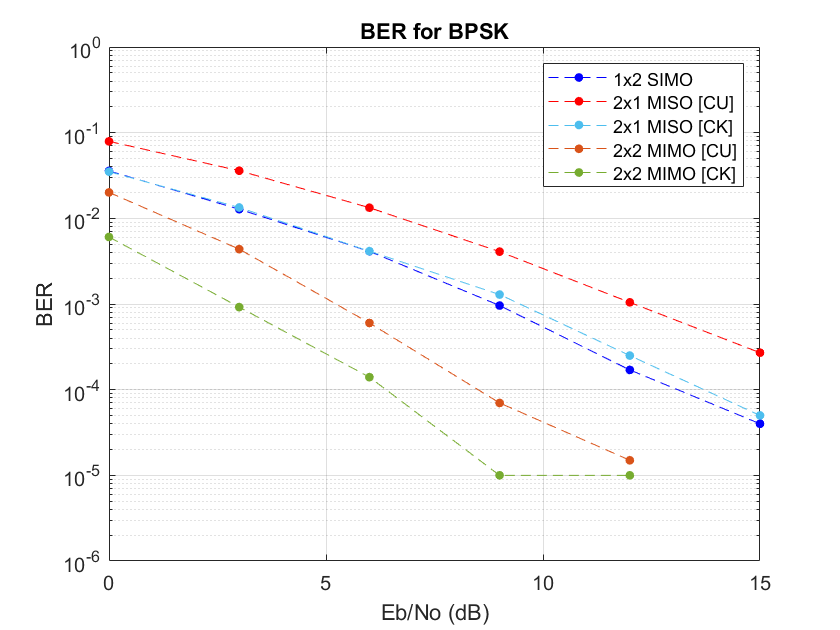
\includegraphics[width=1\textwidth]{2qamber.png}}
		\caption{BER}
	\end{subfigure}%
	\begin{subfigure}{0.5\textwidth}
		\centerline{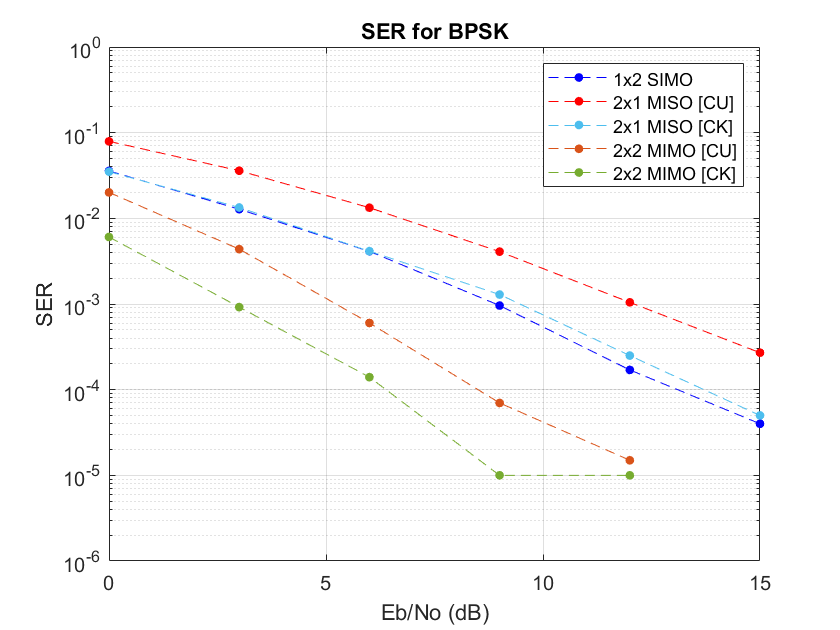
\includegraphics[width=1\textwidth]{2qamser.png}}
		\caption{SER}
	\end{subfigure}\\%
	\caption{}
\end{figure}

\subsubsection{4-QAM}
\begin{figure}[H]
	\centering
	\begin{subfigure}{0.5\textwidth}
		\centerline{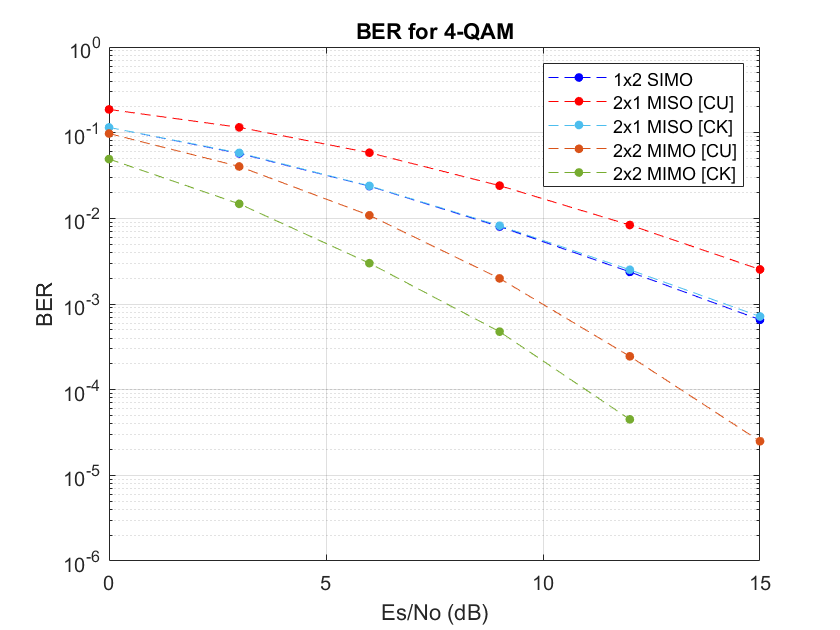
\includegraphics[width=1\textwidth]{4qamber.png}}
		\caption{BER}
	\end{subfigure}%
	\begin{subfigure}{0.5\textwidth}
		\centerline{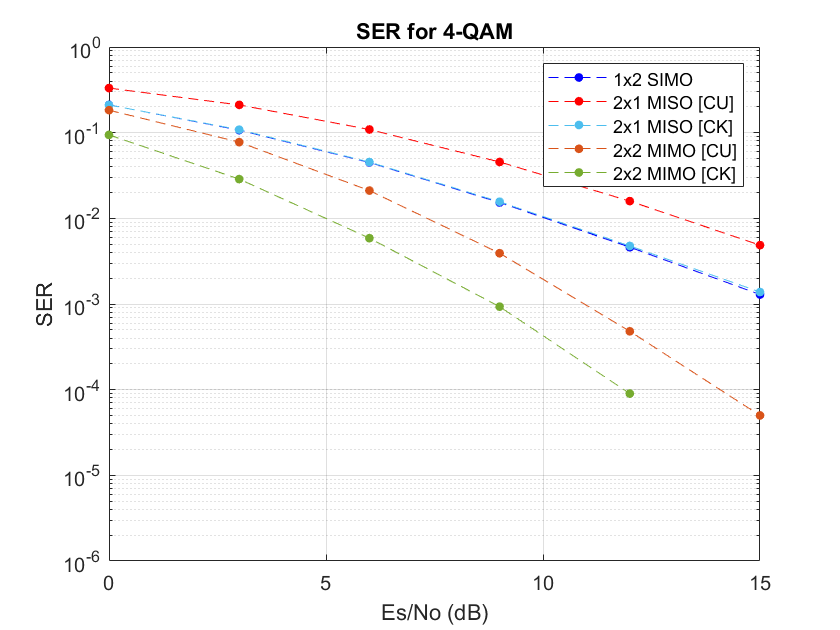
\includegraphics[width=1\textwidth]{4qamser.png}}
		\caption{SER}
	\end{subfigure}\\%
	\begin{subfigure}{0.5\textwidth}
		\centerline{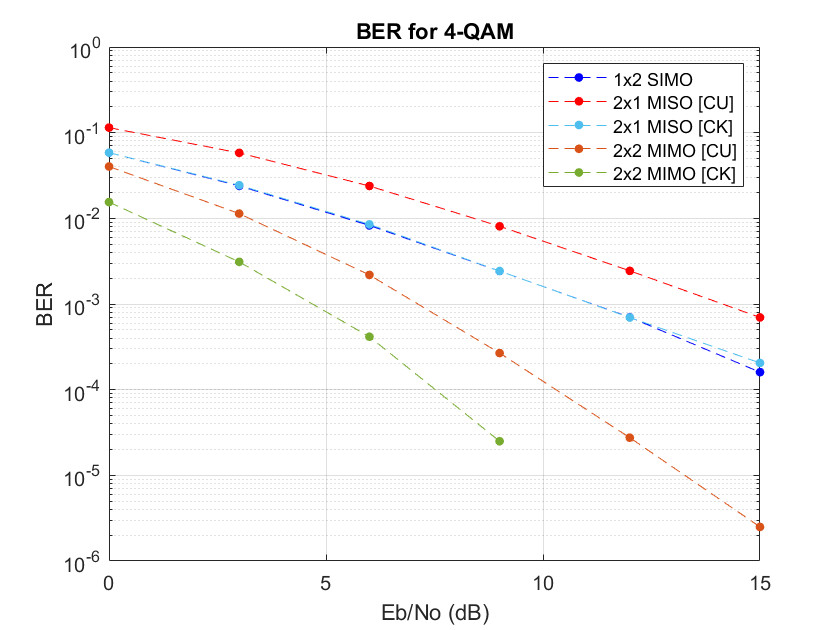
\includegraphics[width=1\textwidth]{4qamber_eb.png}}
		\caption{BER}
	\end{subfigure}%
	\begin{subfigure}{0.5\textwidth}
		\centerline{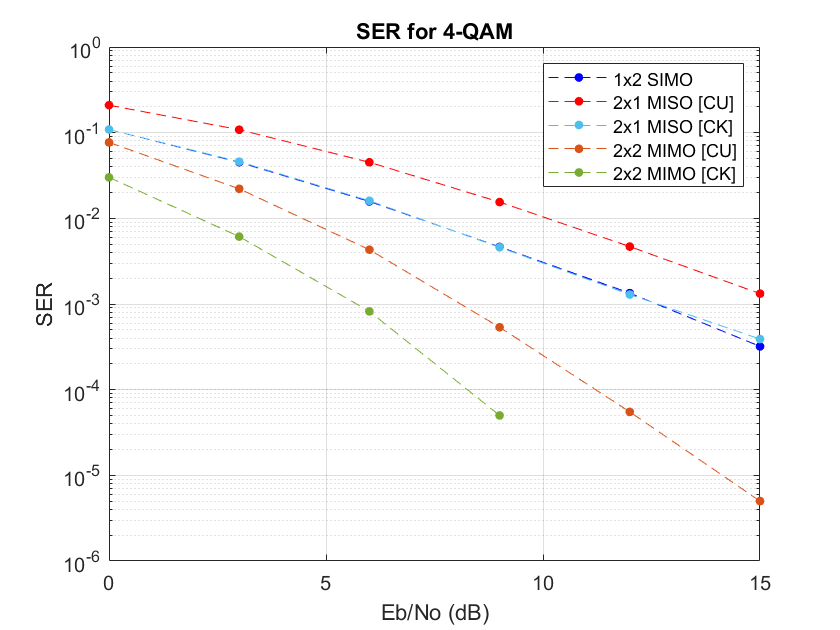
\includegraphics[width=1\textwidth]{4qamser_eb.png}}
		\caption{SER}
	\end{subfigure}\\%
	\caption{}
\end{figure}

\subsubsection{16-QAM}
\begin{figure}[H]
	\centering
	\begin{subfigure}{0.5\textwidth}
		\centerline{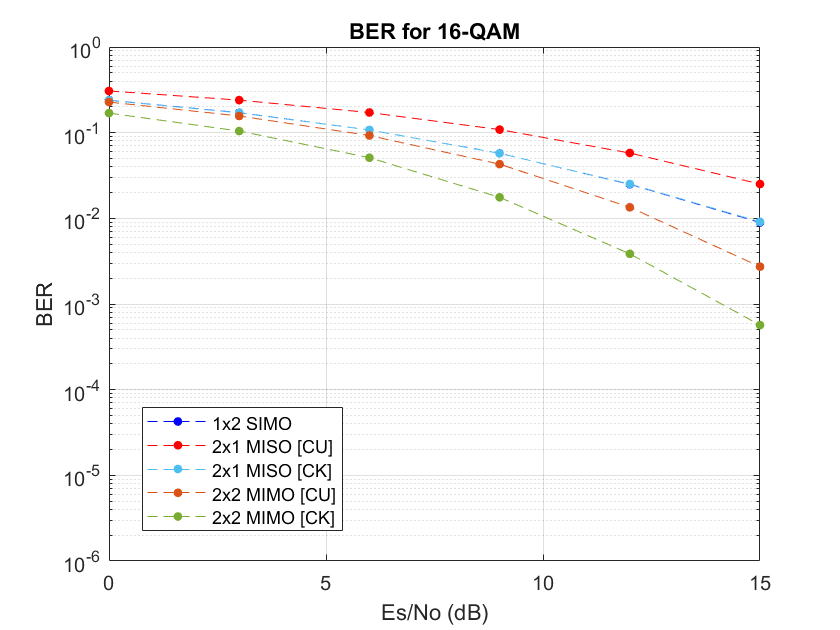
\includegraphics[width=1\textwidth]{16qamber.png}}
		\caption{BER}
	\end{subfigure}%
	\begin{subfigure}{0.5\textwidth}
		\centerline{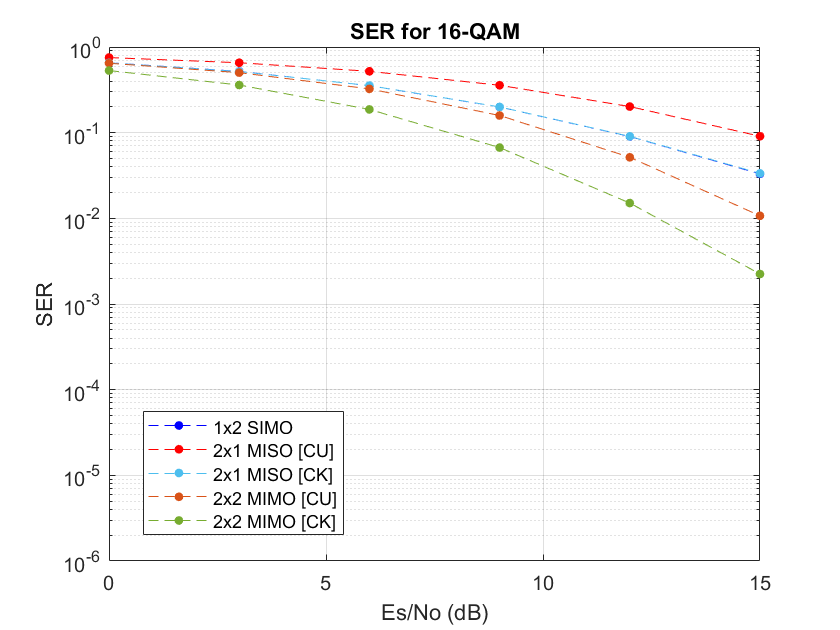
\includegraphics[width=1\textwidth]{16qamser.png}}
		\caption{SER}
	\end{subfigure}\\%
	\begin{subfigure}{0.5\textwidth}
		\centerline{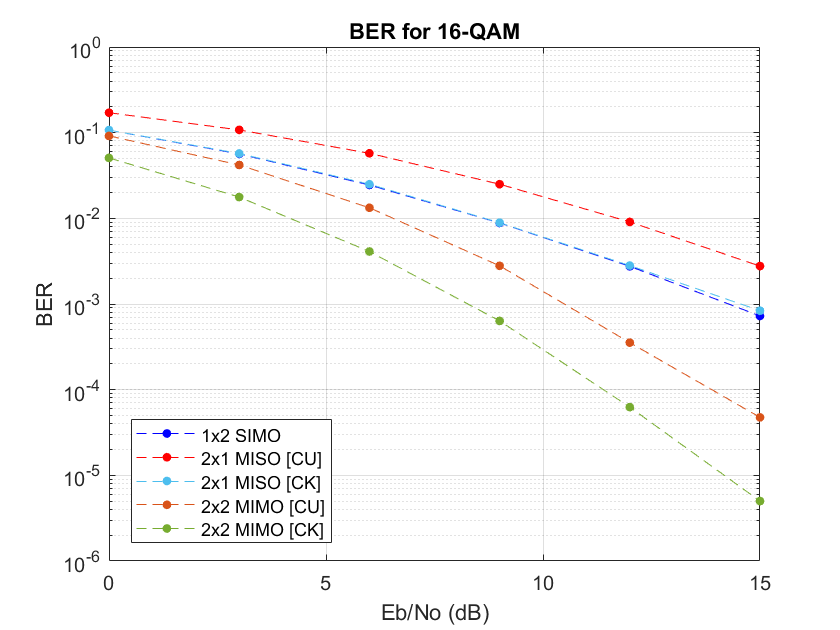
\includegraphics[width=1\textwidth]{16qamber_eb.png}}
		\caption{BER}
	\end{subfigure}%
	\begin{subfigure}{0.5\textwidth}
		\centerline{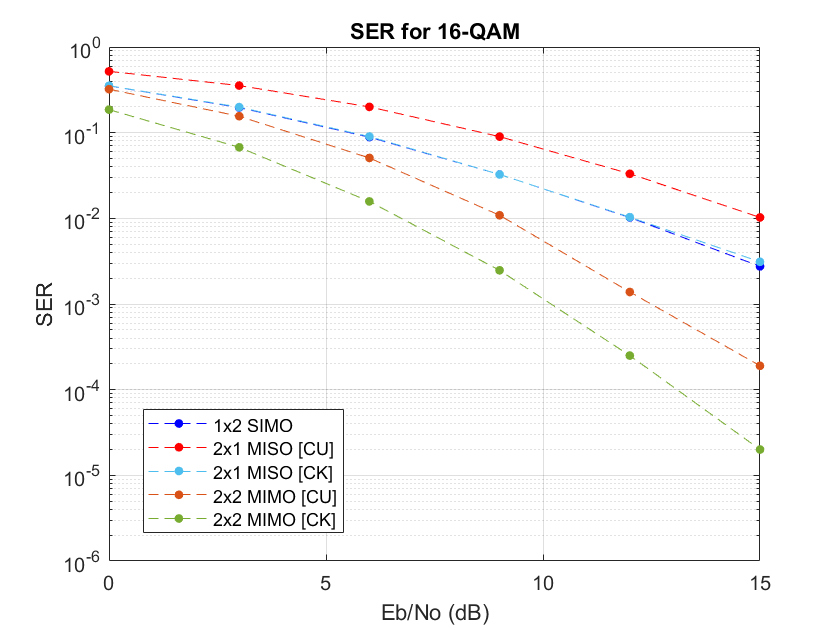
\includegraphics[width=1\textwidth]{16qamser_eb.png}}
		\caption{SER}
	\end{subfigure}\\%
	\caption{}
\end{figure}

\subsection{결과 분석}

\section{개선사항}
\begin{itemize}
	\item 구현은 했으나, Eigenmode decomposition 내용을 정확하게 이해하지 못해 구체적인 분석은 하지 못했다.
\end{itemize}

\section[Entire Code]{Entire Code \footnote{Uploaded on https://github.com/lightwick/ICS$\textunderscore $project/tree/main/Spatial$\textunderscore$Diversity}}
\newgeometry{margin=1cm, bottom=0.5cm}
\noindent\bd{main.m}
\begin{lstlisting}[style=Matlab-editor, frame=single, numbers=left,]
close all
clear all
dbstop if error
% dbstop if warning

addpath('../tools/')

% Environment Varible
M = 4

NumberIteration = 10^5;
SimulationNum = 5;

% Simulation
EbN0_dB = 0:3:15;
EbN0 = db2pow(EbN0_dB);

EsN0 = EbN0 * log2(M);
EsN0_dB = pow2db(EsN0);

% EsN0_dB = 0:3:15;
% EsN0 = db2pow(EsN0_dB);
% 
% EbN0 = EsN0 / log2(M);
% EbN0_dB = pow2db(EbN0);

% BitErrorCount_ZF = zeros(1, length(EsN0_dB));
% SignalErrorCount_ZF = zeros(1, length(EsN0_dB));
% BitErrorCount_MLD = zeros(1, length(EsN0_dB));
% SignalErrorCount_MLD = zeros(1, length(EsN0_dB));
% 33edd
% BitErrorCount_MMSE = zeros(1, length(EsN0_dB));
% SignalErrorCount_MMSE = zeros(1, length(EsN0_dB));

NormalizationFactor = sqrt(2/3*(M-1));

BitErrorCount = zeros(SimulationNum, length(EsN0_dB));
SignalErrorCount = zeros(SimulationNum, length(EsN0_dB));

BEC_tmp = zeros(size(BitErrorCount));
SEC_tmp = zeros(size(SignalErrorCount));
    
FivePercent = ceil(NumberIteration/20);
    
for iTotal = 1 : NumberIteration
    if mod(iTotal-100, FivePercent)==0
        tic
    end
    % Bit Generation
    SignalSequence = randi([0 M-1], 2, 1);
    SignalBinary = de2bi(SignalSequence, log2(M), 'left-msb');
    SymbolSequence = qammod(SignalSequence, M);
%     SymbolSequence = qammod(SignalSequence, M) / NormalizationFactor;
    
    NoiseSequence = (randn(4, 1) + 1j * randn(4, 1)) / sqrt(2); % Noise (n) Generation
%     NoiseSequence = zeros(4,1);
    H = (randn(2, 2) + 1j * randn(2, 2)) ./ sqrt(2); % Receiver x Transmitter

    for indx_EbN0 = 1 : length(EsN0)
        %% SIMO (MRC)
        Nt =1;
        Nr = 2;
        NormalizedSymbol = SymbolSequence(1:Nt, 1) / (NormalizationFactor * sqrt(Nt));
        Noise = NoiseSequence(1:Nr, 1) * sqrt(1 / EsN0(indx_EbN0));

        y = H(1:Nr, 1:Nt) * NormalizedSymbol + Noise;
        [BEC_tmp(1, indx_EbN0), SEC_tmp(1, indx_EbN0)] = simo_mrc(y, SignalSequence(1:Nt,1), SignalBinary(1:Nt, :),  M, H(1:Nr, 1:Nt));
        
        %% MISO (Alamouti)
        Nt = 2;
        Nr = 1;
        NormalizedSymbol = SymbolSequence(1:Nt, 1)/ (NormalizationFactor * sqrt(Nt));
        % Row prepresents antenna, Column represents time-slot
        STBC = [NormalizedSymbol.'; -conj(NormalizedSymbol(2,1)) conj(NormalizedSymbol(1,1))].';
        y_alamouti = (H(1:Nr, 1:Nt) * STBC).' + NoiseSequence(1:Nt, 1) * sqrt(1 / EsN0(indx_EbN0));
        
        [BEC_tmp(2, indx_EbN0), SEC_tmp(2, indx_EbN0)] = miso_alamouti(y_alamouti, SignalSequence(1:Nt, 1), SignalBinary(1:Nt, :),  M, H(1:Nr,1:Nt));
        
        %% MISO (MRT)
        Nt = 2;
        Nr = 1;
        H_new = H(1:Nr,1:Nt);
        [BEC_tmp(3, indx_EbN0), SEC_tmp(3, indx_EbN0)] = miso_mrt(SymbolSequence(1), SignalSequence(1), Noise(1:Nr), SignalBinary(1, :), M, H_new);

        %% MIMO (Alamouti)
        Nt = 2;
        Nr = 2;
        NormalizedSymbol = SymbolSequence(1:Nt, 1)/ (NormalizationFactor * sqrt(Nt));
        % Row prepresents antenna, Column represents time-slot
        STBC = [NormalizedSymbol.'; -conj(NormalizedSymbol(2,1)) conj(NormalizedSymbol(1,1))].';
        Hs = reshape((H(1:Nr, 1:Nt) * STBC), [], 1);
        y_alamouti = Hs + NoiseSequence * sqrt(1 / EsN0(indx_EbN0));
        [BEC_tmp(4, indx_EbN0), SEC_tmp(4, indx_EbN0)] = mimo_alamouti(y_alamouti, SignalSequence(1:Nt, 1), SignalBinary(1:Nt, :),  M, H(1:Nr, 1:Nt));
        
        %% MIMO (MRT)
        Nt = 2;
        Nr = 2;
        H_new = H(1:Nr,1:Nt);
        Noise = NoiseSequence(1:Nr, 1) * sqrt(1 / EsN0(indx_EbN0));
        [BEC_tmp(5, indx_EbN0), SEC_tmp(5, indx_EbN0)] = mimo_mrt(SymbolSequence(1), SignalSequence(1), Noise(1:Nr), SignalBinary(1, :), M, H_new);
    end
    
    BitErrorCount = BitErrorCount + BEC_tmp;
    SignalErrorCount = SignalErrorCount + SEC_tmp;
    
    if mod(iTotal-100, FivePercent)==0
        ElapsedTime = toc;
        EstimatedTime = (NumberIteration-iTotal)*ElapsedTime;
        disp(sprintf("%d%%, estimated wait time %d minutes %d seconds", round(iTotal/NumberIteration*100), floor(EstimatedTime/60), floor(mod(EstimatedTime, 60))))
    end
end

BER = BitErrorCount / (NumberIteration*log2(M));
SER = SignalErrorCount / (NumberIteration);

BER(2,:) = BER(2,:) / 2;
SER(2,:) = SER(2,:) / 2

BER(4,:) = BER(4,:) / 2;
SER(4,:) = SER(4,:) / 2;

% Plot
BER_Title = sprintf("BER for %d-QAM", M);
SER_Title = sprintf("SER for %d-QAM", M);
x_axis = "Eb/No (dB)";

legend_order = ["1x2 SIMO", "2x1 MISO [CU]", "2x1 MISO [CK]", "2x2 MIMO [CU]", "2x2 MIMO [CK]"];
myplot(EbN0_dB, BER, BER_Title, x_axis, "BER", legend_order);
ylim([10^(-6) 1])
myplot(EbN0_dB, SER, SER_Title, x_axis, "SER", legend_order);
ylim([10^(-6) 1])
\end{lstlisting}
\noindent
\bd{simo$\textunderscore$mrc.m}
\begin{lstlisting}[style=Matlab-editor, frame=single, numbers=left,]
function [BitErrorCount, SignalErrorCount] = simo_mrc(ReceivedSymbolSequence, SignalSequence, SignalBinary,  M, H)
    Nt = size(H,2);
    Nr = size(H,1);
    assert(Nt==1, 'Nt is not 1')
    NormalizationFactor = sqrt(2/3*(M-1) * Nt);
    
    y = ReceivedSymbolSequence;
    z = H'*y;
    
    DetectedSignal = qamdemod(z/norm(H,'fro')^2*NormalizationFactor, M);
    DetectedBinary = de2bi(DetectedSignal, log2(M), 'left-msb');
    
    SignalErrorCount = sum(DetectedSignal~=SignalSequence, 'all');
    BitErrorCount = sum(SignalBinary~=DetectedBinary, 'all');
end
\end{lstlisting}
\bd{miso$\textunderscore$alamouti.m}
\begin{lstlisting}[style=Matlab-editor, frame=single, numbers=left,]
function [BitErrorCount, SignalErrorCount] = miso_alamouti(ReceivedSymbolSequence, SignalSequence, SignalBinary,  M, H)
    Nt = size(H,2);
    Nr = size(H,1);
    assert(Nt==2 && Nr==1, "Need H of size 1x2")
    
    Augmented_H = [H; conj(H(1,2)) -conj(H(1,1))];
    
    NormalizationFactor = sqrt(2/3*(M-1) * Nt);
    
    y = [ReceivedSymbolSequence(1,1); conj(ReceivedSymbolSequence(2,1))];
    z = Augmented_H' * y;
    
    FrobSquared = H*H'; % equivalent to norm(H,'fro')^2
    DetectedSignal = qamdemod(z/FrobSquared*NormalizationFactor, M);
    DetectedBinary = de2bi(DetectedSignal, log2(M), 'left-msb');
    
    SignalErrorCount = sum(DetectedSignal~=SignalSequence, 'all');
    BitErrorCount = sum(SignalBinary~=DetectedBinary, 'all');
end
\end{lstlisting}
\bd{miso$\textunderscore$mrt.m}
\begin{lstlisting}[style=Matlab-editor, frame=single, numbers=left,]
function [BitErrorCount, SignalErrorCount] = miso_mrt(SymbolSequence, SignalSequence, Noise, SignalBinary,  M, H)
    Nt = size(H,2);
    Nr = size(H,1);
    assert(Nt==2 && Nr==1, "Need H of size 1x2")

    NormalizationFactor = sqrt(2/3*(M-1) * norm(H, "fro")^2);
    w = H';
    TransmitSymbol = w * SymbolSequence / NormalizationFactor;
    ReceivedSymbol = H*TransmitSymbol + Noise;

    FrobSquared = H*H'; % equivalent to norm(H,'fro')^2
    DetectedSignal = qamdemod(ReceivedSymbol/FrobSquared*NormalizationFactor, M);
    DetectedBinary = de2bi(DetectedSignal, log2(M), 'left-msb');
    
    SignalErrorCount = sum(DetectedSignal~=SignalSequence, 'all');
    BitErrorCount = sum(SignalBinary~=DetectedBinary, 'all');
end
\end{lstlisting}
\bd{mimo$\textunderscore$alamouti.m}
\begin{lstlisting}[style=Matlab-editor, frame=single, numbers=left,]
function [BitErrorCount, SignalErrorCount] = mimo_alamouti(y, SignalSequence, SignalBinary,  M, H)
    Nt = size(H,2);
    Nr = size(H,1);
    assert(Nt==2 && Nr==2, 'H is not size 2x2')
    assert(length(SignalSequence), "Signal Sequence is not 2")

    tmp_H = conj(H(:,[2 1]));
    tmp_H(:,2) = -tmp_H(:,2);

    Augmented_H = [H; tmp_H];
    NormalizationFactor = sqrt(2/3*(M-1) * Nt);
    
    y([3 4], :) = conj(y([3 4], :));
    z = Augmented_H' * y;
    FrobSquared = norm(H,'fro')^2;
    
    DetectedSignal = qamdemod(z/FrobSquared*NormalizationFactor, M);
    DetectedBinary = de2bi(DetectedSignal, log2(M), 'left-msb');
    
    SignalErrorCount = sum(DetectedSignal~=SignalSequence, 'all');
    BitErrorCount = sum(SignalBinary~=DetectedBinary, 'all');
end
\end{lstlisting}
\bd{mimo$\textunderscore$mrt.m}
\begin{lstlisting}[style=Matlab-editor, frame=single, numbers=left,]
function [BitErrorCount, SignalErrorCount] = mimo_mrt(SymbolSequence, SignalSequence, Noise, SignalBinary,  M, H)
    Nt = size(H,2);
    Nr = size(H,1);
    
    % S = svd(A) returns the singular values of matrix A in descending order.
    [U,S,V] = svd(H);
    w =V(:,1);
    g = U(:,1);
    
    NormalizationFactor = sqrt(2/3*(M-1));
    TransmitSymbol = w * SymbolSequence / NormalizationFactor;
    ReceivedSymbol = H * TransmitSymbol + Noise;

    Processing = g' * ReceivedSymbol;
    
    DetectedSignal = qamdemod(Processing/S(1,1)*NormalizationFactor, M);
    DetectedBinary = de2bi(DetectedSignal, log2(M), 'left-msb');
    
    SignalErrorCount = sum(DetectedSignal~=SignalSequence, 'all');
    BitErrorCount = sum(SignalBinary~=DetectedBinary, 'all');
end
\end{lstlisting}
\end{document}